\mode*

\section{Disposition}

\begin{frame}
  \begin{figure}
    \includegraphics[height=0.8\textheight]{fig/book.jpg}
    \caption{Front cover of Necessary Conditions of Learning.}
  \end{figure}
\end{frame}

\begin{frame}
  \begin{enumerate}
    \item What makes humans human?
    \alert{\item What is to be learned?}
    \item Sameness and difference in learning
    \item What does the world look like to others?
    \item The art of learning
    \item Making learning possible
    \item Learning to help others to learn
  \end{enumerate}
\end{frame}

\begin{frame}
  \begin{block}{Ch 2 What is to be learned?}
    \begin{itemize}
      \item What is an intended learning outcome?
      \item What should it be?
      \item It depends on the learner: \emph{critical aspects, critical 
        features} --- the atoms of the learning objective.
    \end{itemize}
  \end{block}
  
  \pause

  \begin{remark}[The goal]
    \begin{itemize}
      \item \textcquote{NecessaryConditionsOfLearning}{The focus of the theory 
        elaborated in this book is on learning to handle new situations in 
      powerful ways.}
    \end{itemize}
  \end{remark}
\end{frame}

\section{Intended learning outcomes}

\begin{frame}
  \begin{example}[Answers to \enquote{what's to be learned?}]
    \begin{description}
      \item[Subject content] \eg
        quadratic equations.

      \item[Educational objective] (or \emph{intended learning outcome}) \eg
        solve problems requiring quadratic equations.

      \item[Intended object of learning] \eg
        what quadratic equations have non-real roots.

      \item[Enacted object of learning] \eg
        \enquote{hopefully} what quadratic equations have non-real roots,
        but maybe only \emph{that} quadratic equations have non-real roots.

      \item[Lived object of learning] \eg
        \enquote{hopefully} what quadratic equations have non-real roots,
        but maybe only that some quadratic equations can't be solved.
    \end{description}
  \end{example}
\end{frame}

\begin{frame}
  \begin{example}[Answers to \enquote{what's to be learned?}]
    \begin{description}
      \item[Subject content] \dots
      \item[Educational objective] (or \emph{intended learning outcome}) \dots
      \item[Intended object of learning] \dots
        critical aspects
      \item[Enacted object of learning] \dots
        critical aspects
      \item[Lived object of learning] \dots
        critical aspects
    \end{description}
  \end{example}

  \begin{remark}[By {\cite[Ch.~7, p.~277]{NecessaryConditionsOfLearning}}]
    \begin{itemize}
      \item As teachers become better teachers, their focus progress down this 
        list.
    \end{itemize}
  \end{remark}
\end{frame}

\begin{frame}
  \begin{center}
    Transition from\\[0.5em]
    What is to be done?\\[0.5em]
    towards\\[0.5em]
    What is to be learned?
  \end{center}
\end{frame}

\section{Critial aspects and features}

\begin{frame}
  \begin{figure}
    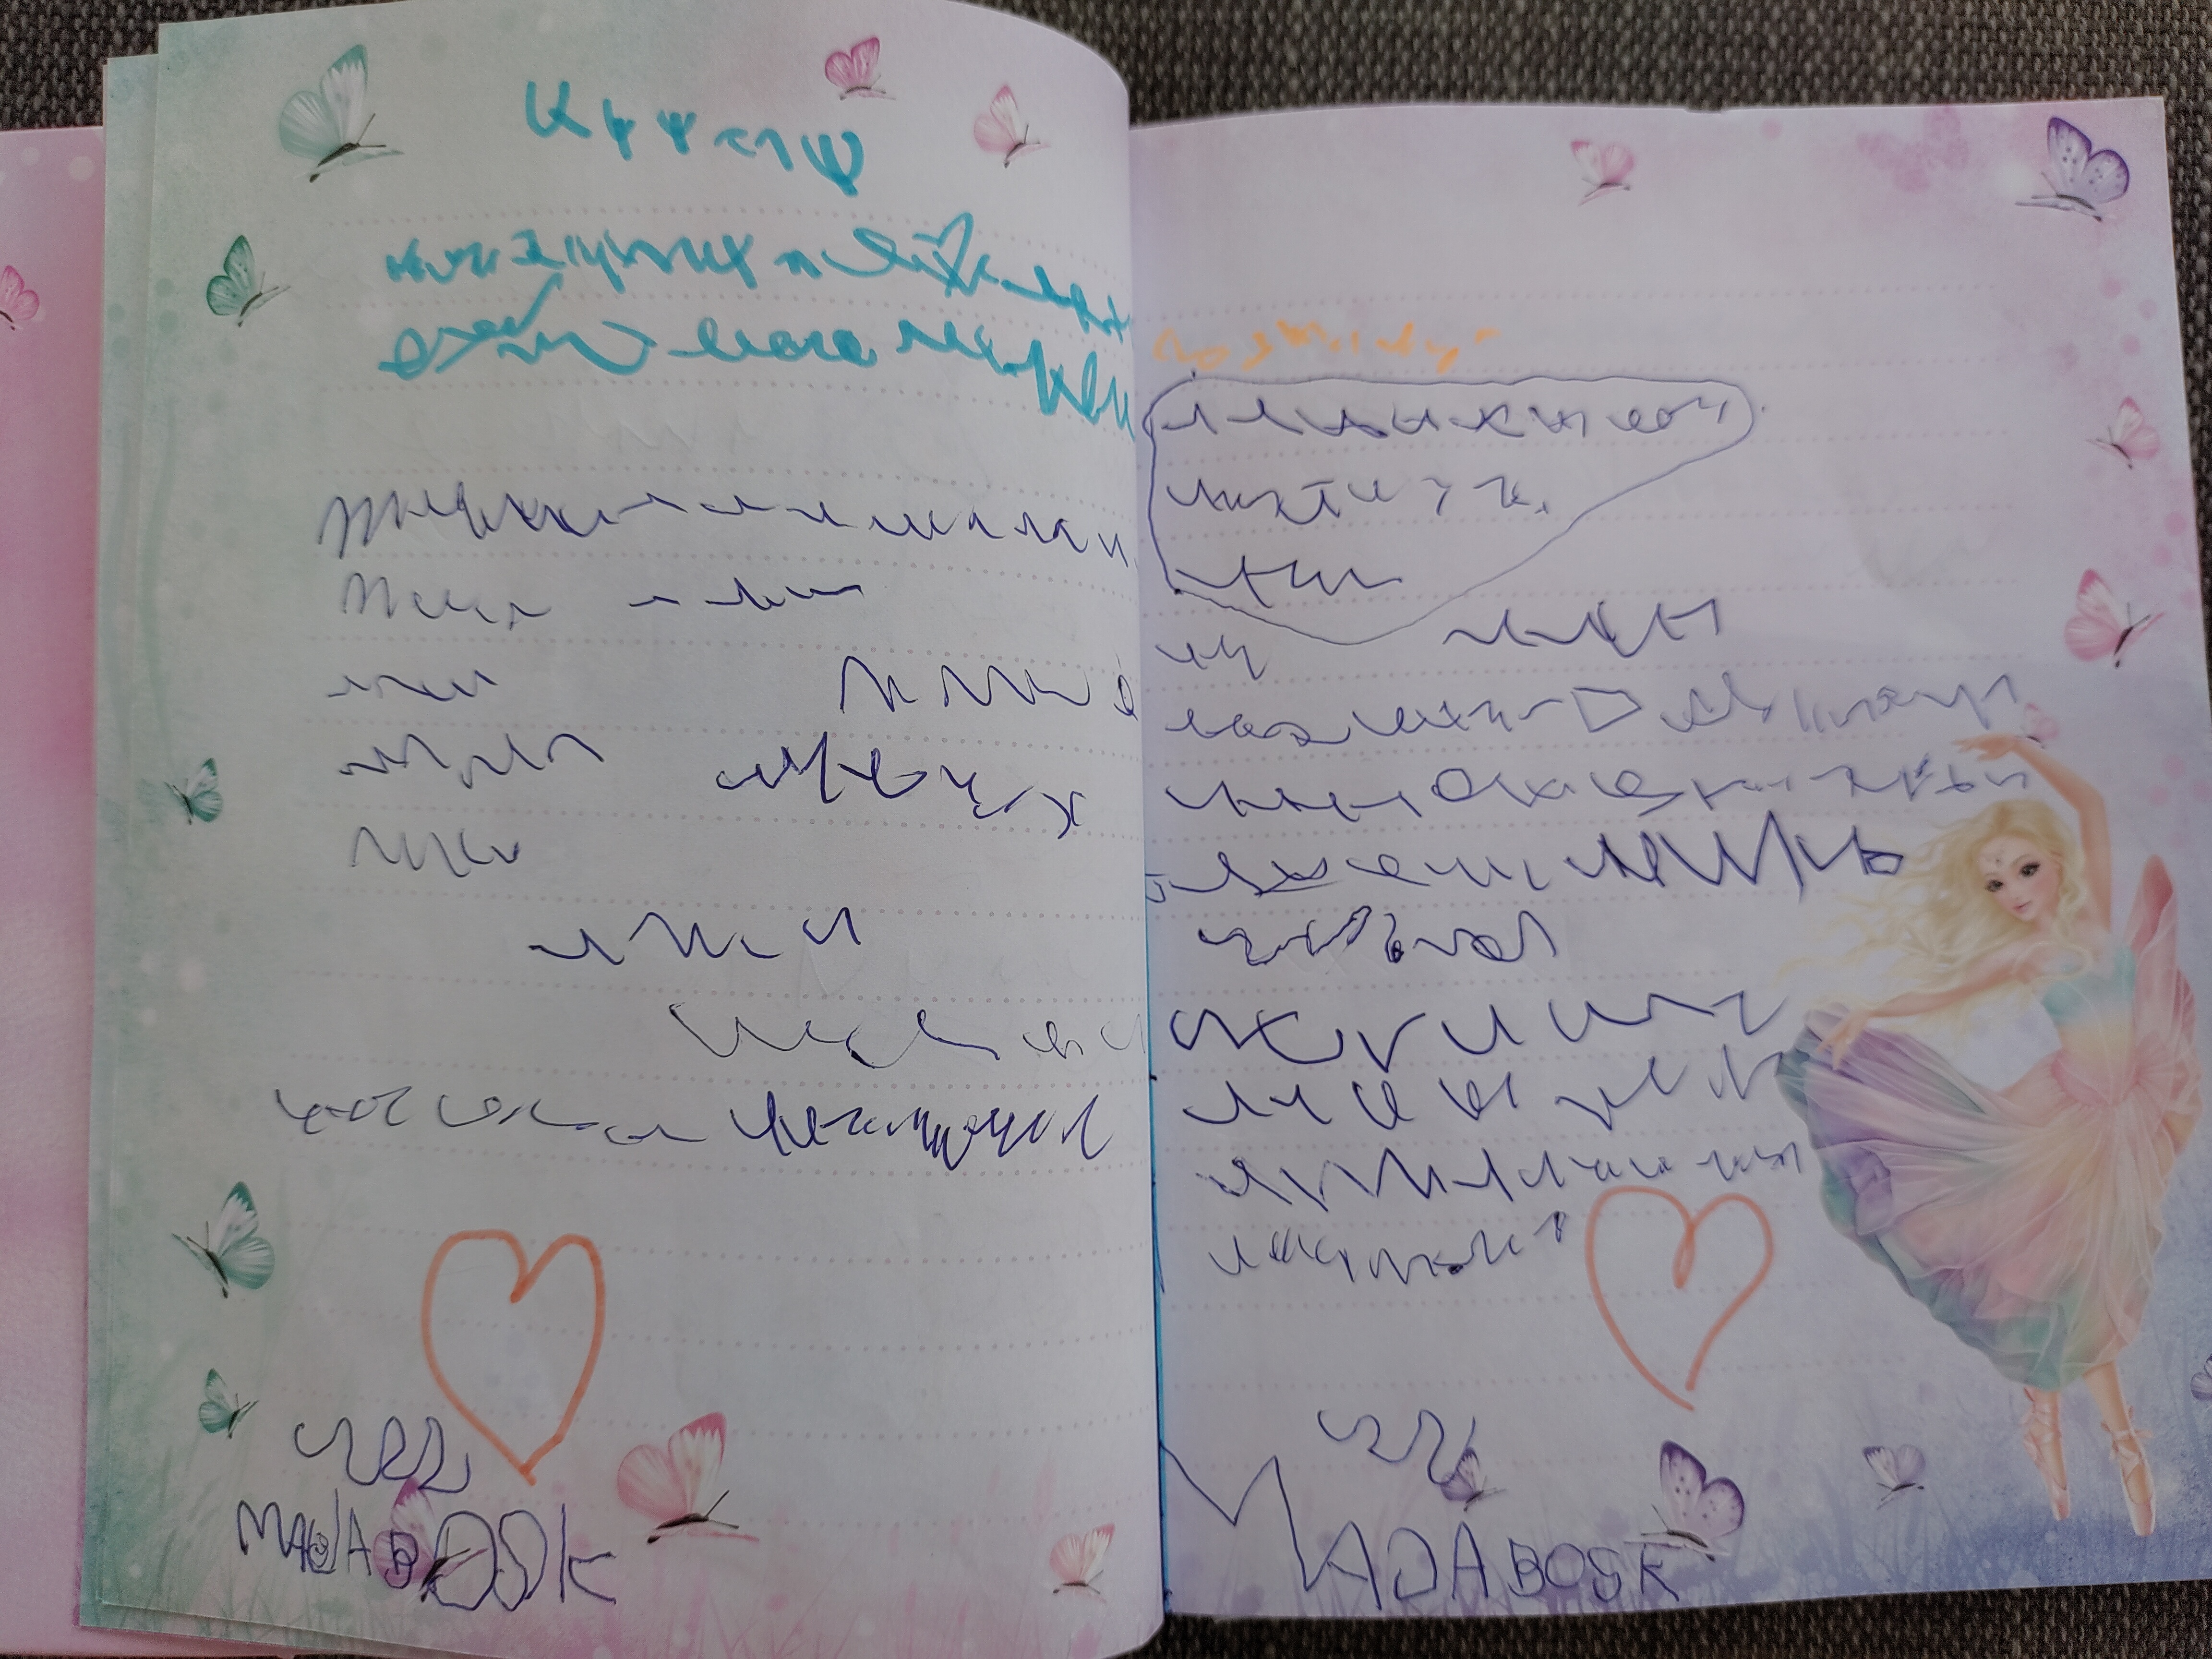
\includegraphics[height=0.5\textheight]{fig/maja-writing.png}
    \caption{My daughter's writing. (Corresponds to~\cite[Fig.~2.1, 
    p.~30]{NecessaryConditionsOfLearning}.)}
  \end{figure}
  \begin{example}
    \begin{itemize}
      \item Obviously my daughter knows some aspect(s) of writing.
      \item Just not all that are needed.
    \end{itemize}
  \end{example}
\end{frame}

\begin{frame}
  \begin{remark}
    \begin{itemize}
      \item Eventually she learned more aspects of reading and writing.
      \item One at a time \dots
    \end{itemize}
  \end{remark}

  \begin{figure}
    \includegraphics[height=0.5\textheight]{fig/papaebest.jpg}
    \caption{The aspect of characters mapping to sounds.}
  \end{figure}
\end{frame}

\begin{frame}[fragile]
  \begin{example}[Programming]
    \inputminted{python}{scope.py}
  \end{example}
\end{frame}

\begin{frame}
  \blockcquote[p.~37]{NecessaryConditionsOfLearning}
  {%
    The object of learning \textelp{} amounts to becoming able to discern all 
    the critical aspects and to focus on them simultaneously.%
  }
\end{frame}

